% \newcommand{\undersetimage}[3]{
    \begin{tikzpicture}
        \node[anchor=south west,inner sep=0] (image) at (0, 0)
            {\includegraphics[width=0.65cm]{#1}};
        \begin{scope}[x={(image.south east)},y={(image.north west)}]
            \node[] at (0.5, #3) {#2};
        \end{scope}
    \end{tikzpicture}
}

\begin{figure*}
\centering
\begin{minipage}[t]{0.55\textwidth}
    \raisebox{2cm}{\textbf{a}}~~~
    \hspace{.2cm}
    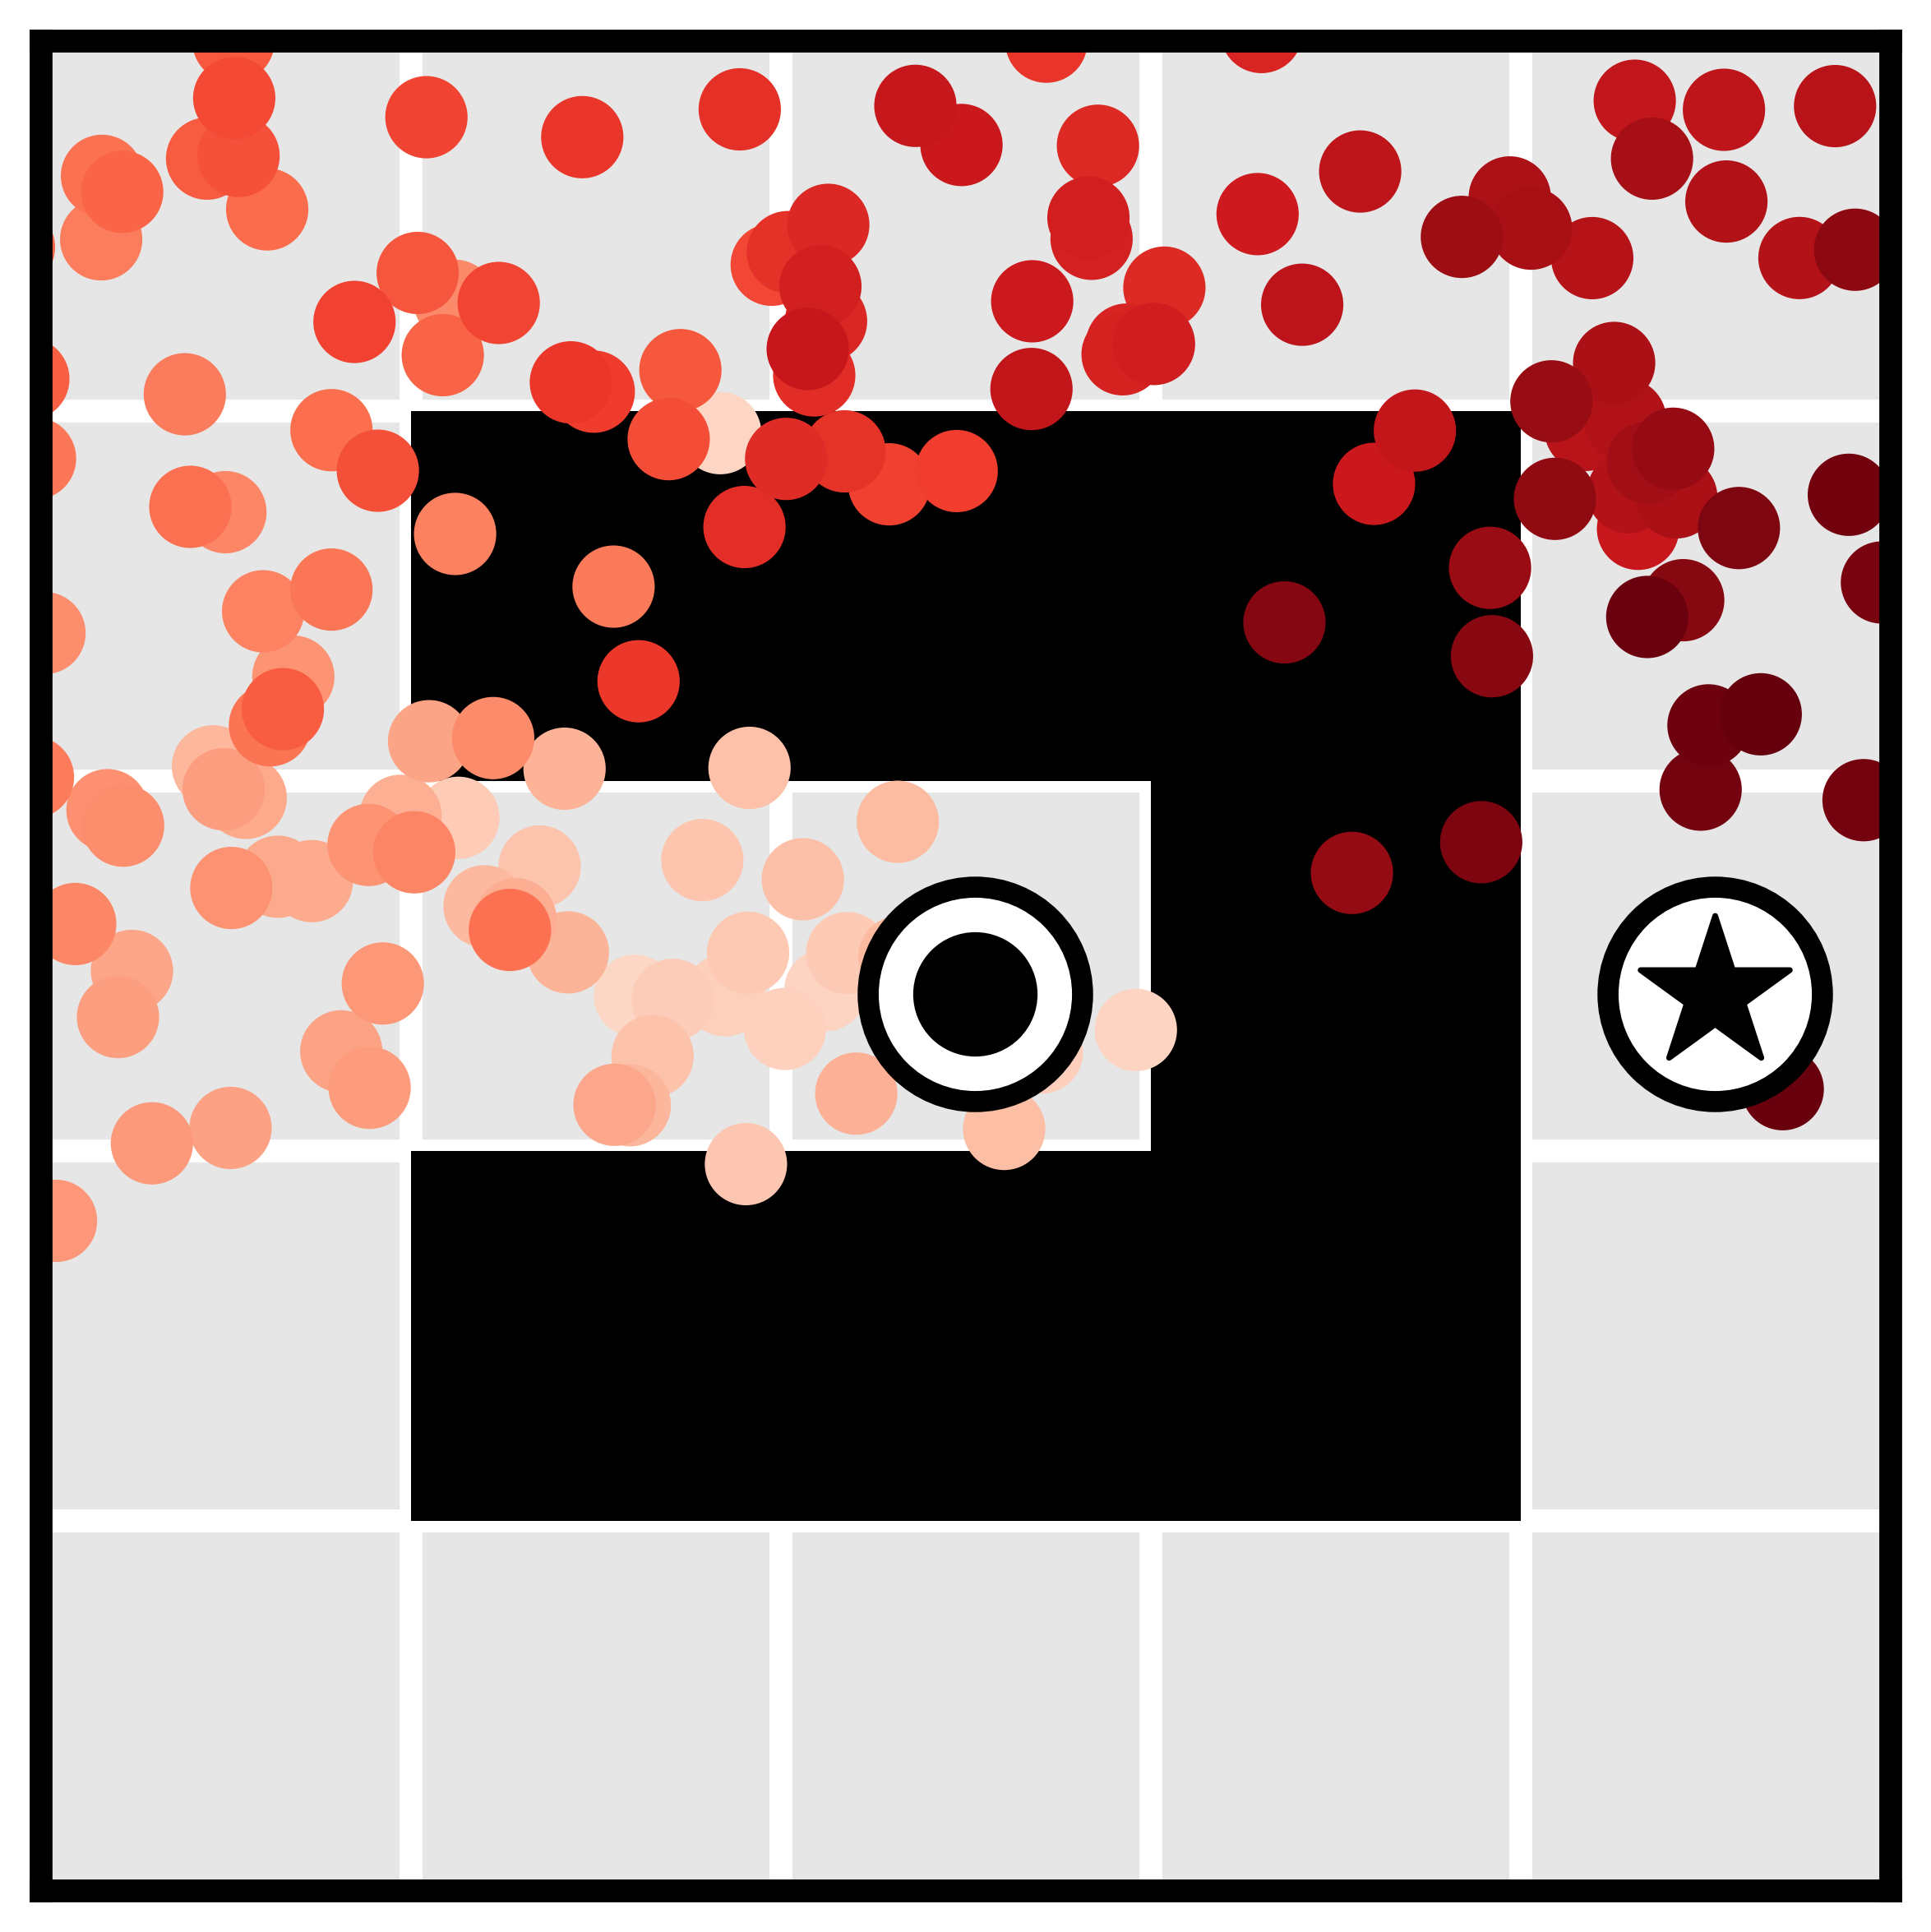
\includegraphics[width=2.5cm]{images/properties/planning_2.png}~
    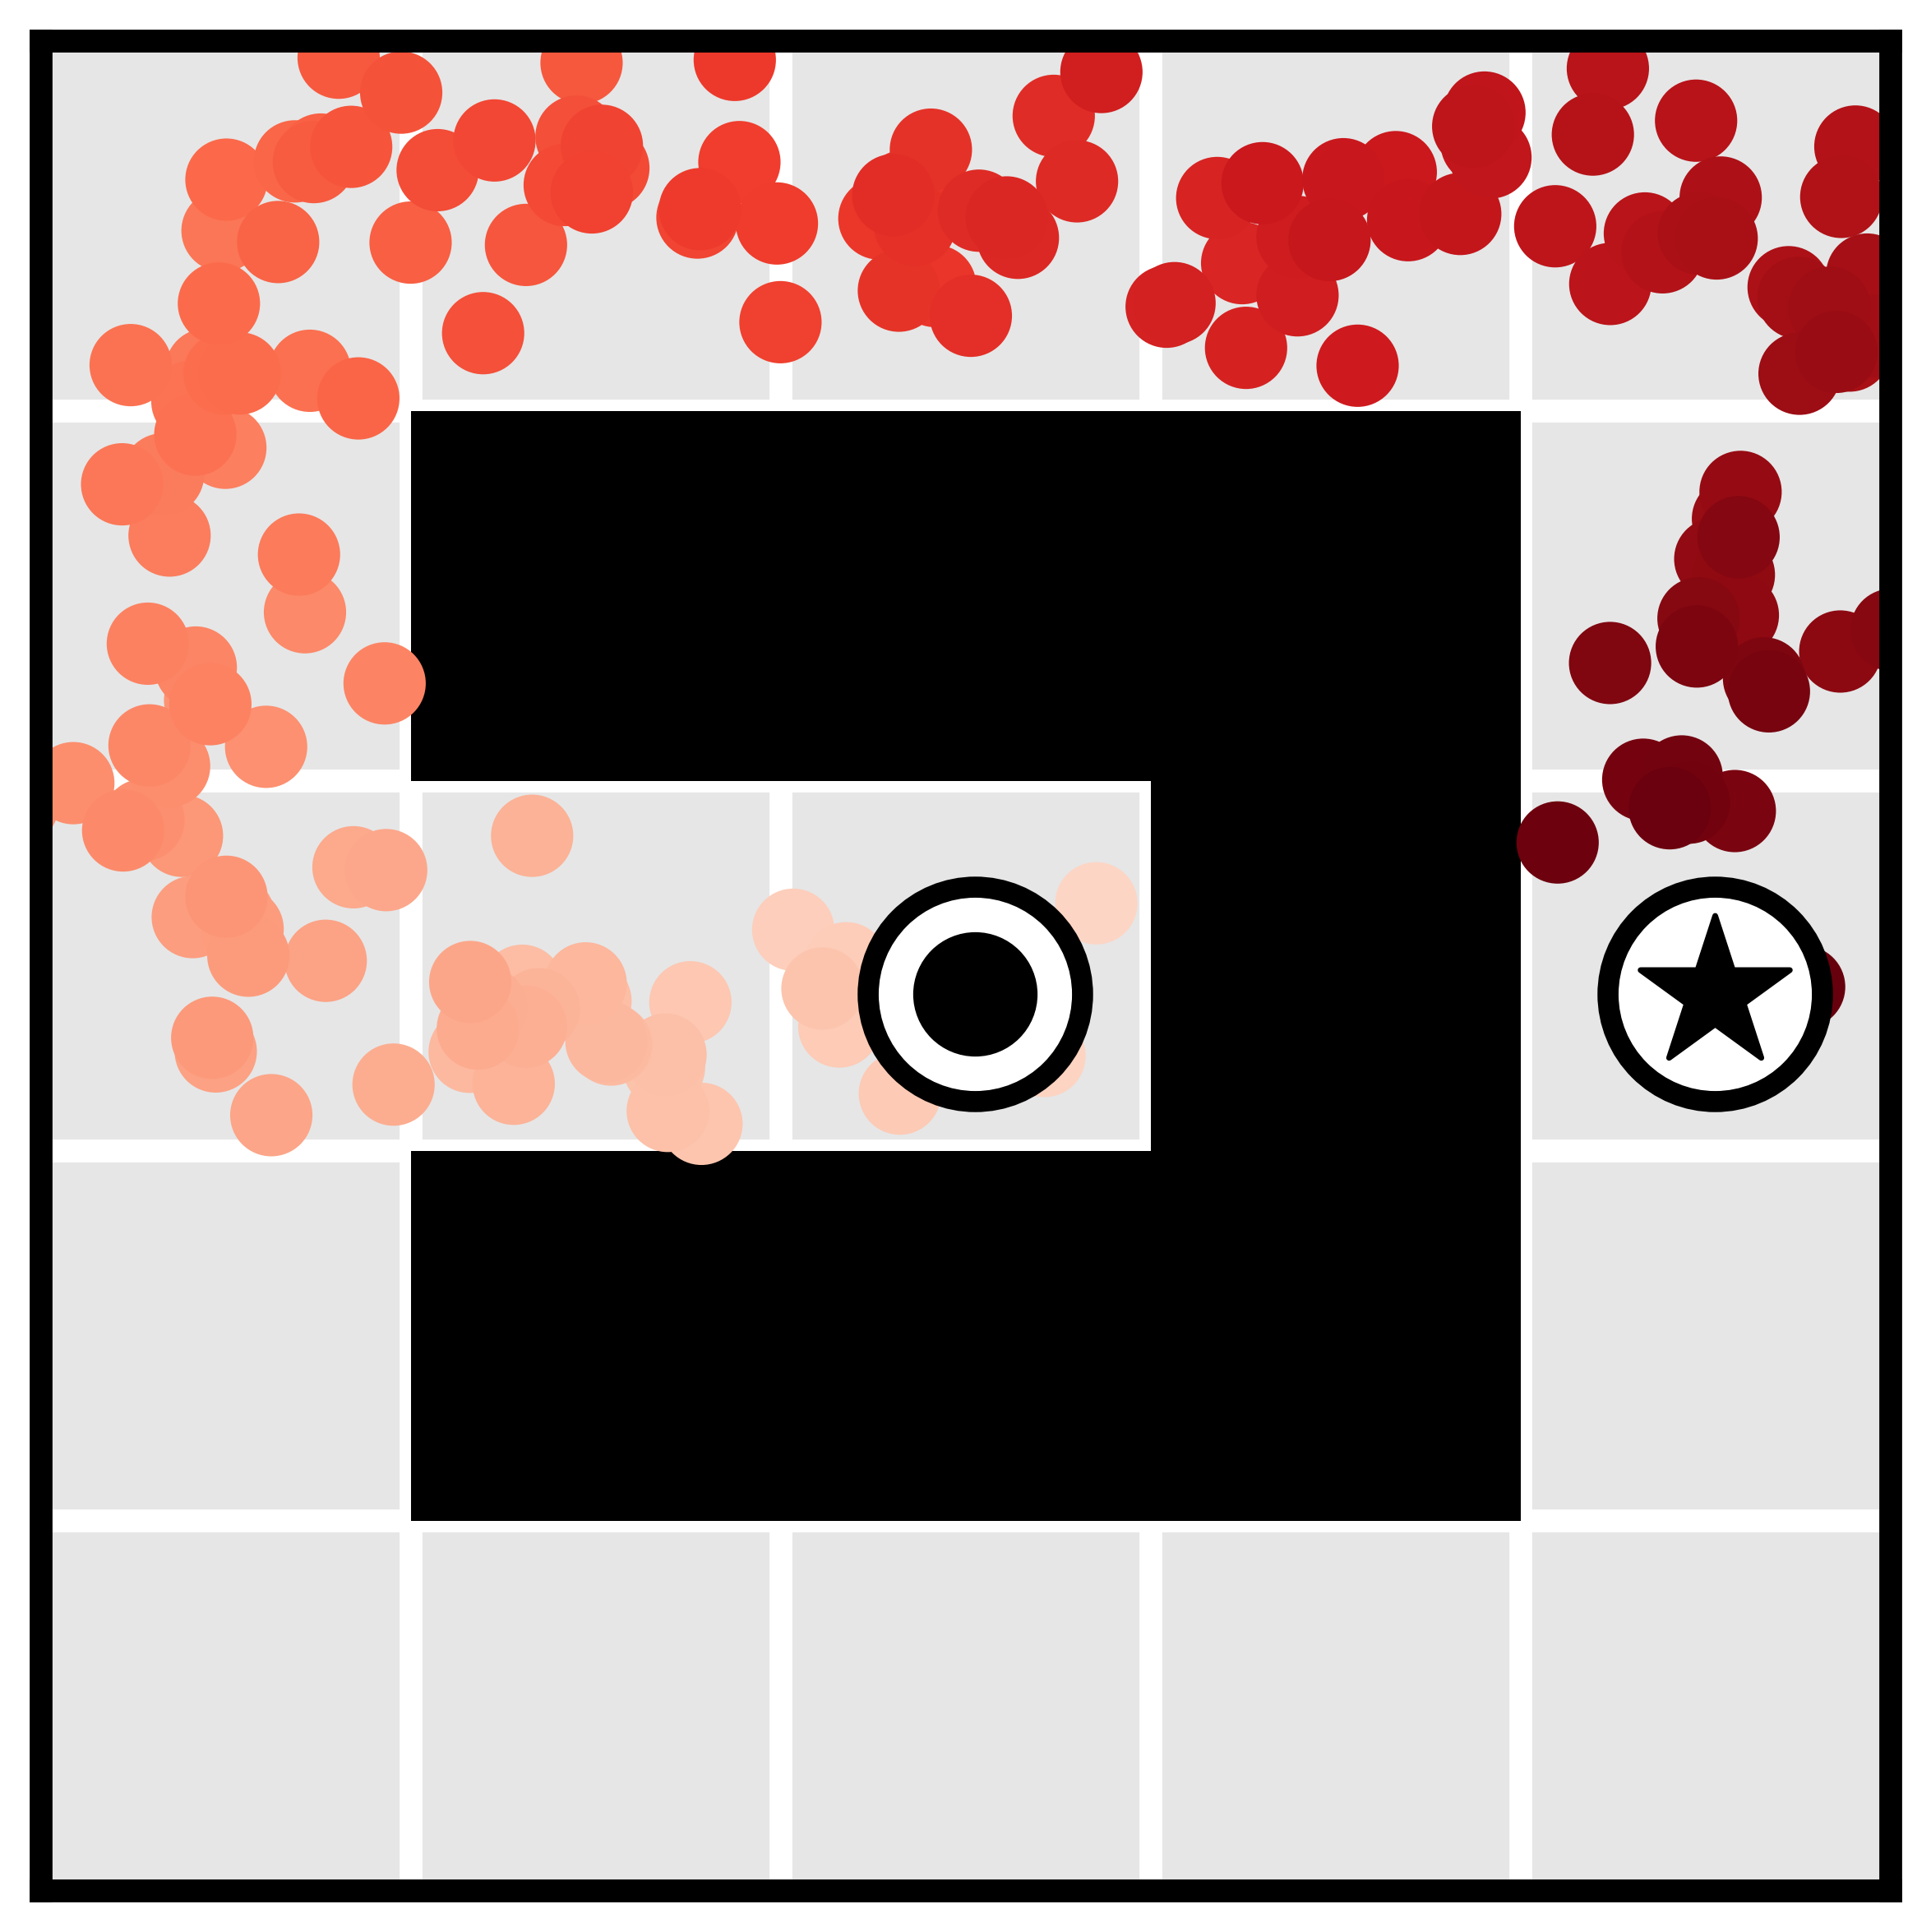
\includegraphics[width=2.5cm]{images/properties/planning_1.png}~
    
\includegraphics[width=2.5cm]{images/properties/planning_0.png} \\
    \vspace{-.4cm}
    \begin{center}
        \raisebox{.3\height}{denoising}~~
        \tikz \draw [-{Computer Modern Rightarrow[length=1.33mm, width=2mm]}, line width=.2mm] (0,0) -- (3,0); \\
    \end{center}
\end{minipage}%
%%%%
\begin{minipage}[t]{0.35\textwidth}
    \raisebox{2cm}{\textbf{b}}~~~
    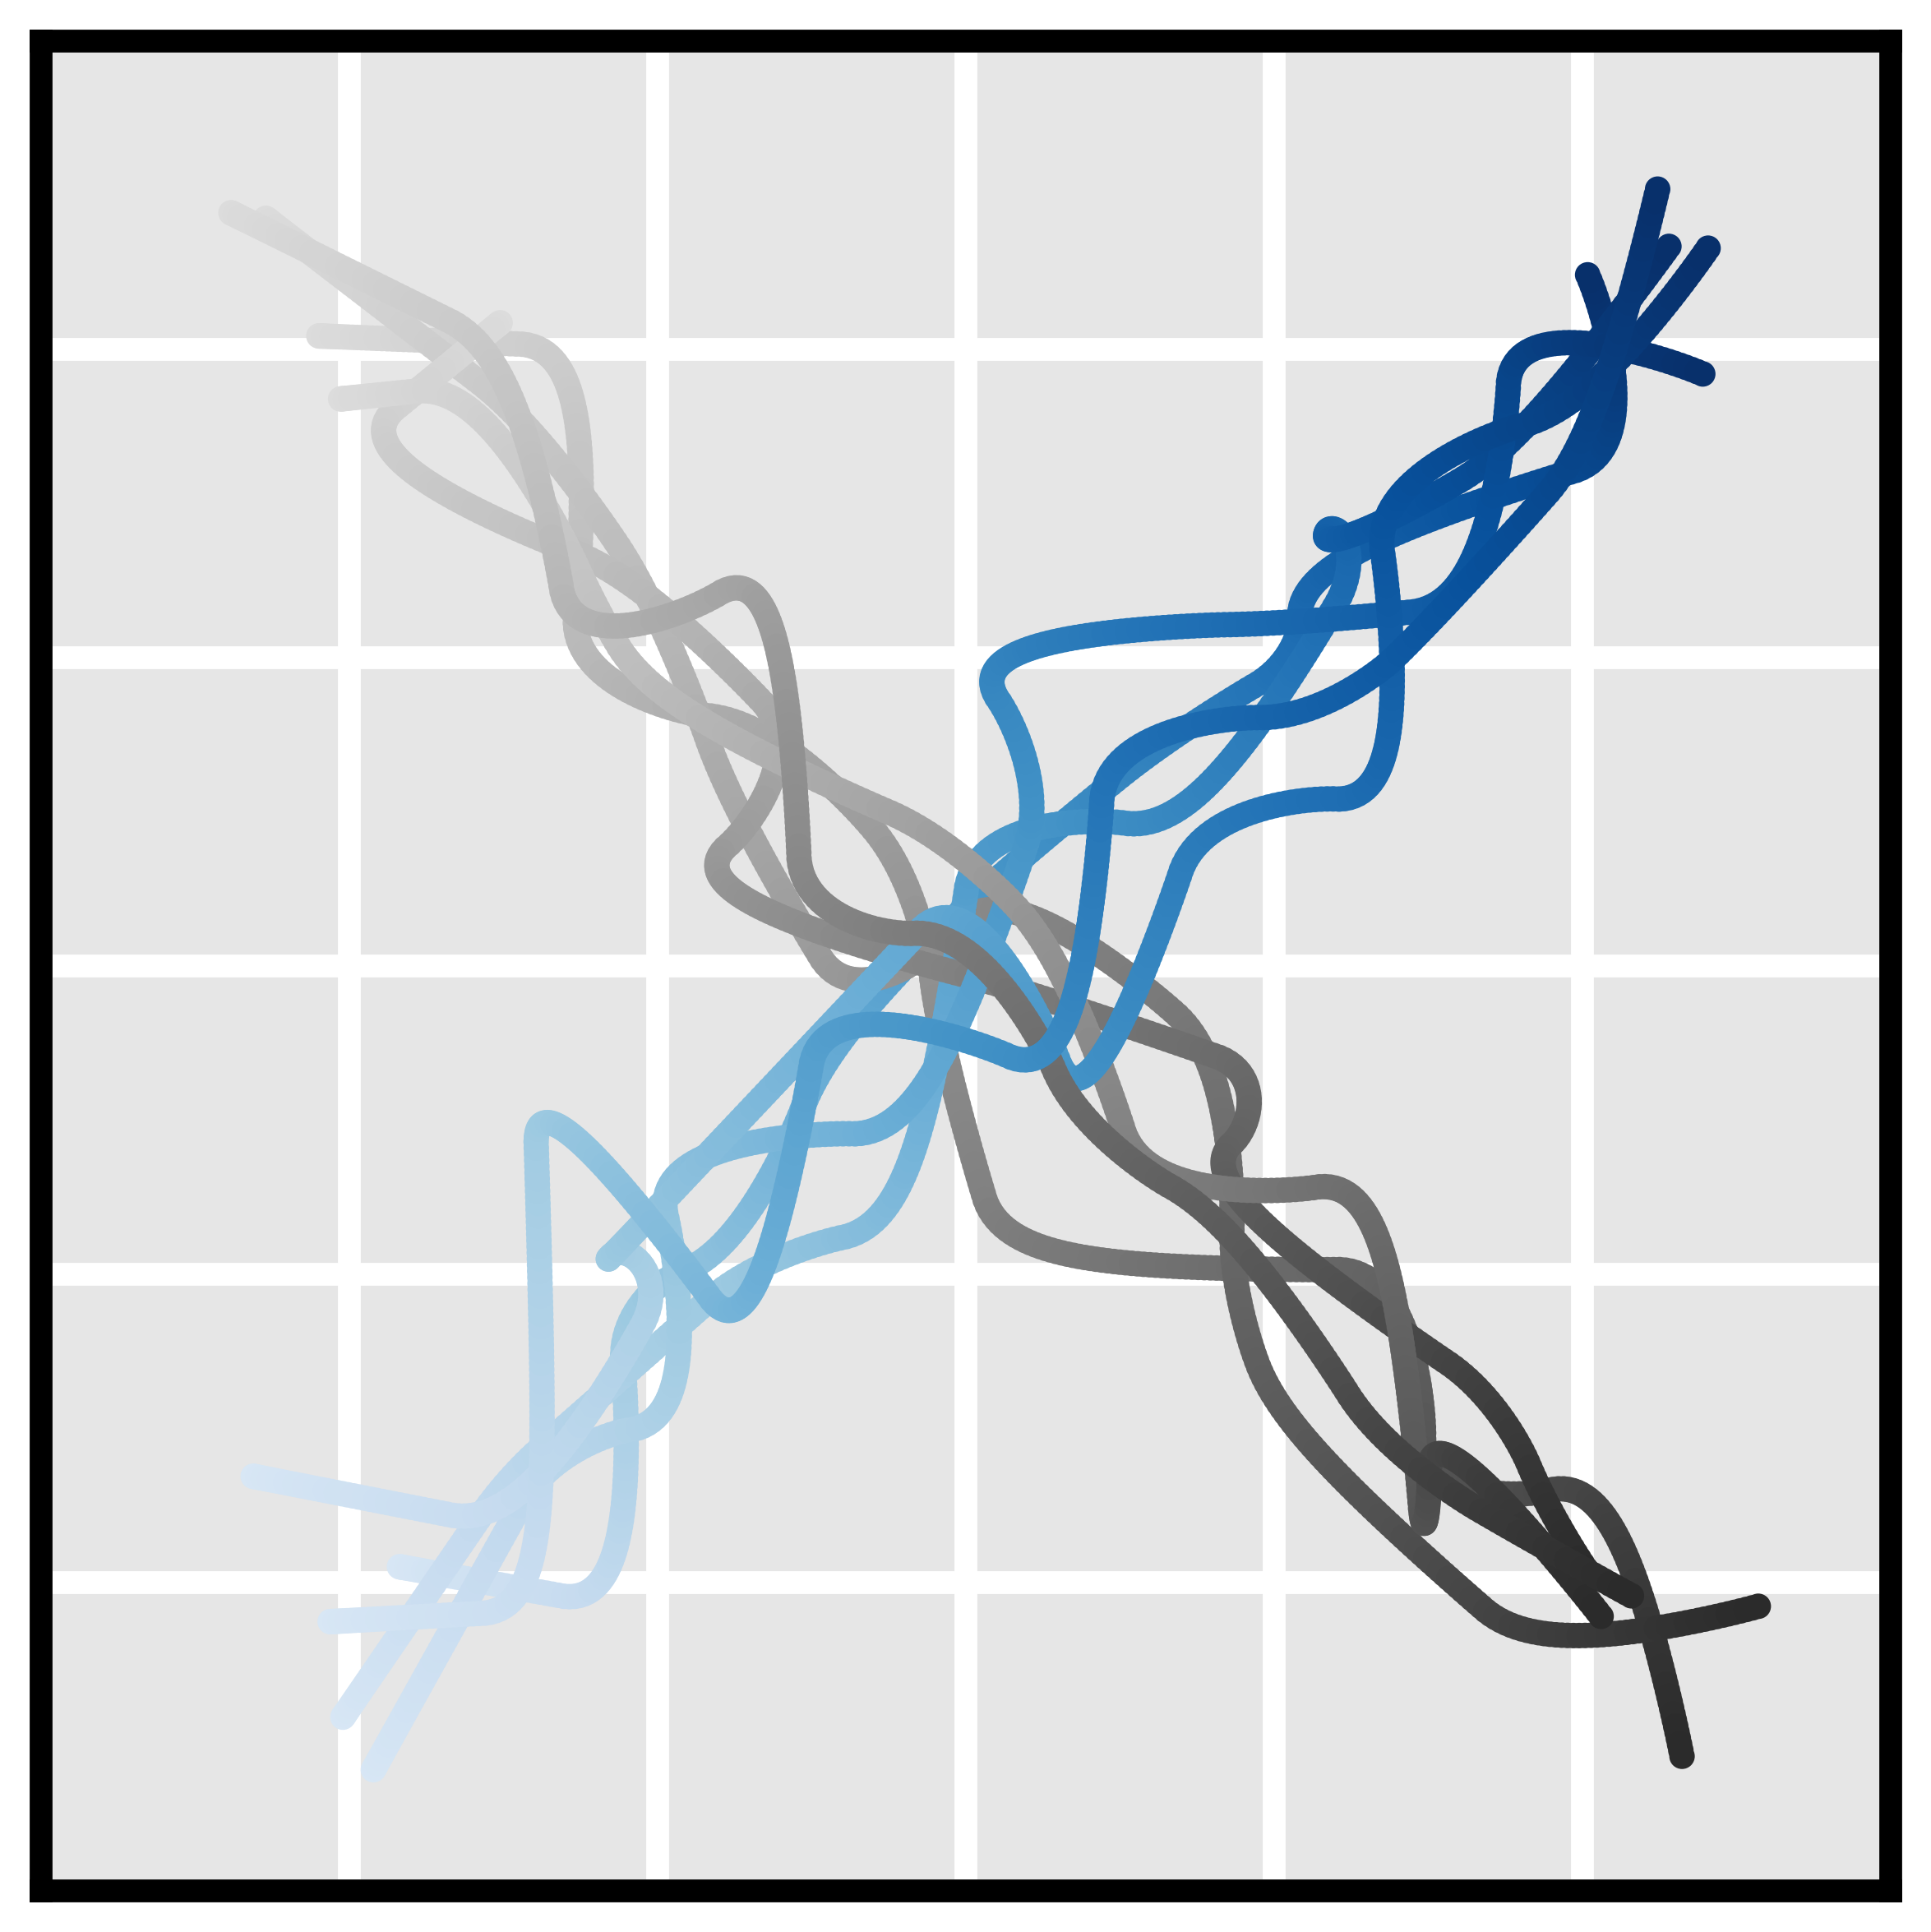
\includegraphics[width=2.5cm]{images/properties/stitching_data.png}~
    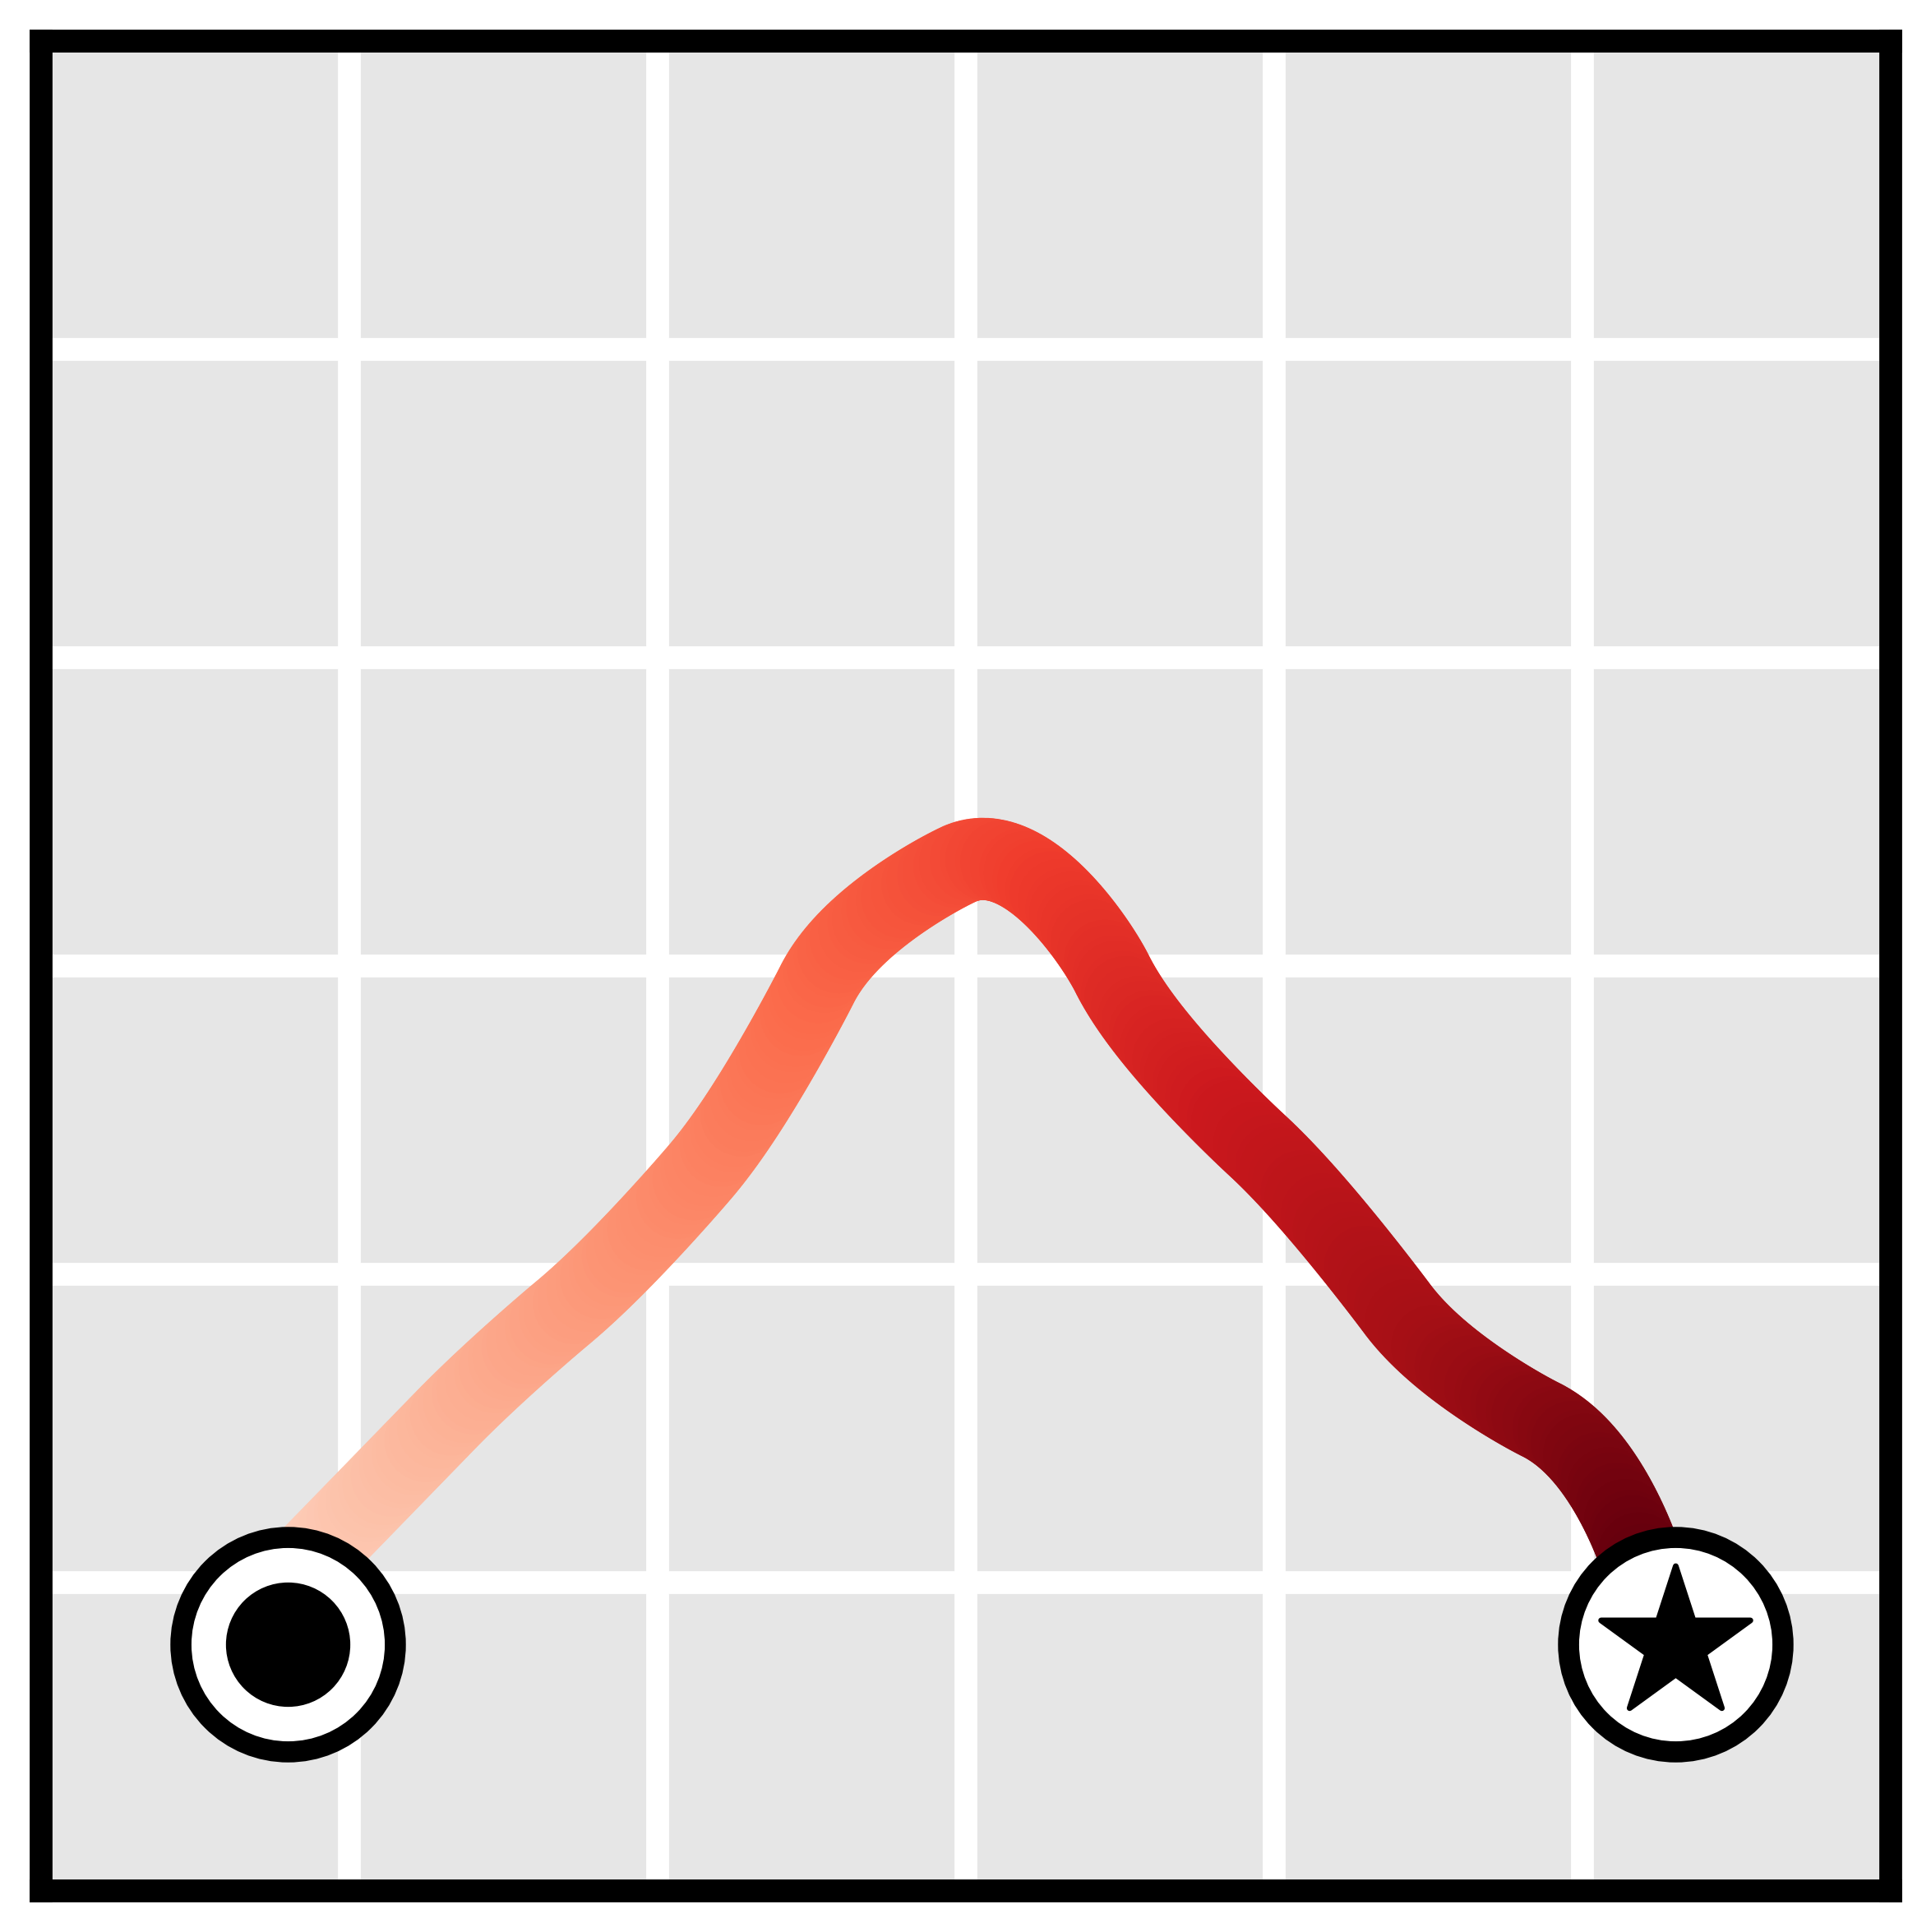
\includegraphics[width=2.5cm]{images/properties/stitching_plan.png} \\
    \vspace{-.5cm}
    \begin{center}
            \hspace{0.1cm} data \hspace{1.8cm} plan \\
    \end{center}
\end{minipage} \\
\vspace{.4cm}
%%%%
\begin{minipage}[t]{0.55\textwidth}
    \raisebox{2cm}{\textbf{c}}~~~
    \raisebox{0.3cm}{\undersetimage{images/properties/rand_0.png}{$\btau{N}$}{-0.25}}
        \raisebox{1.2cm}{$\rightarrow$}
        
\includegraphics[width=2.5cm]{images/properties/variable_0.png}
        ~~
    \raisebox{-0.1cm}{\undersetimage{images/properties/rand_1.png}{$\btau{N}$}{-0.15}}
        \raisebox{1.2cm}{$\rightarrow$}
        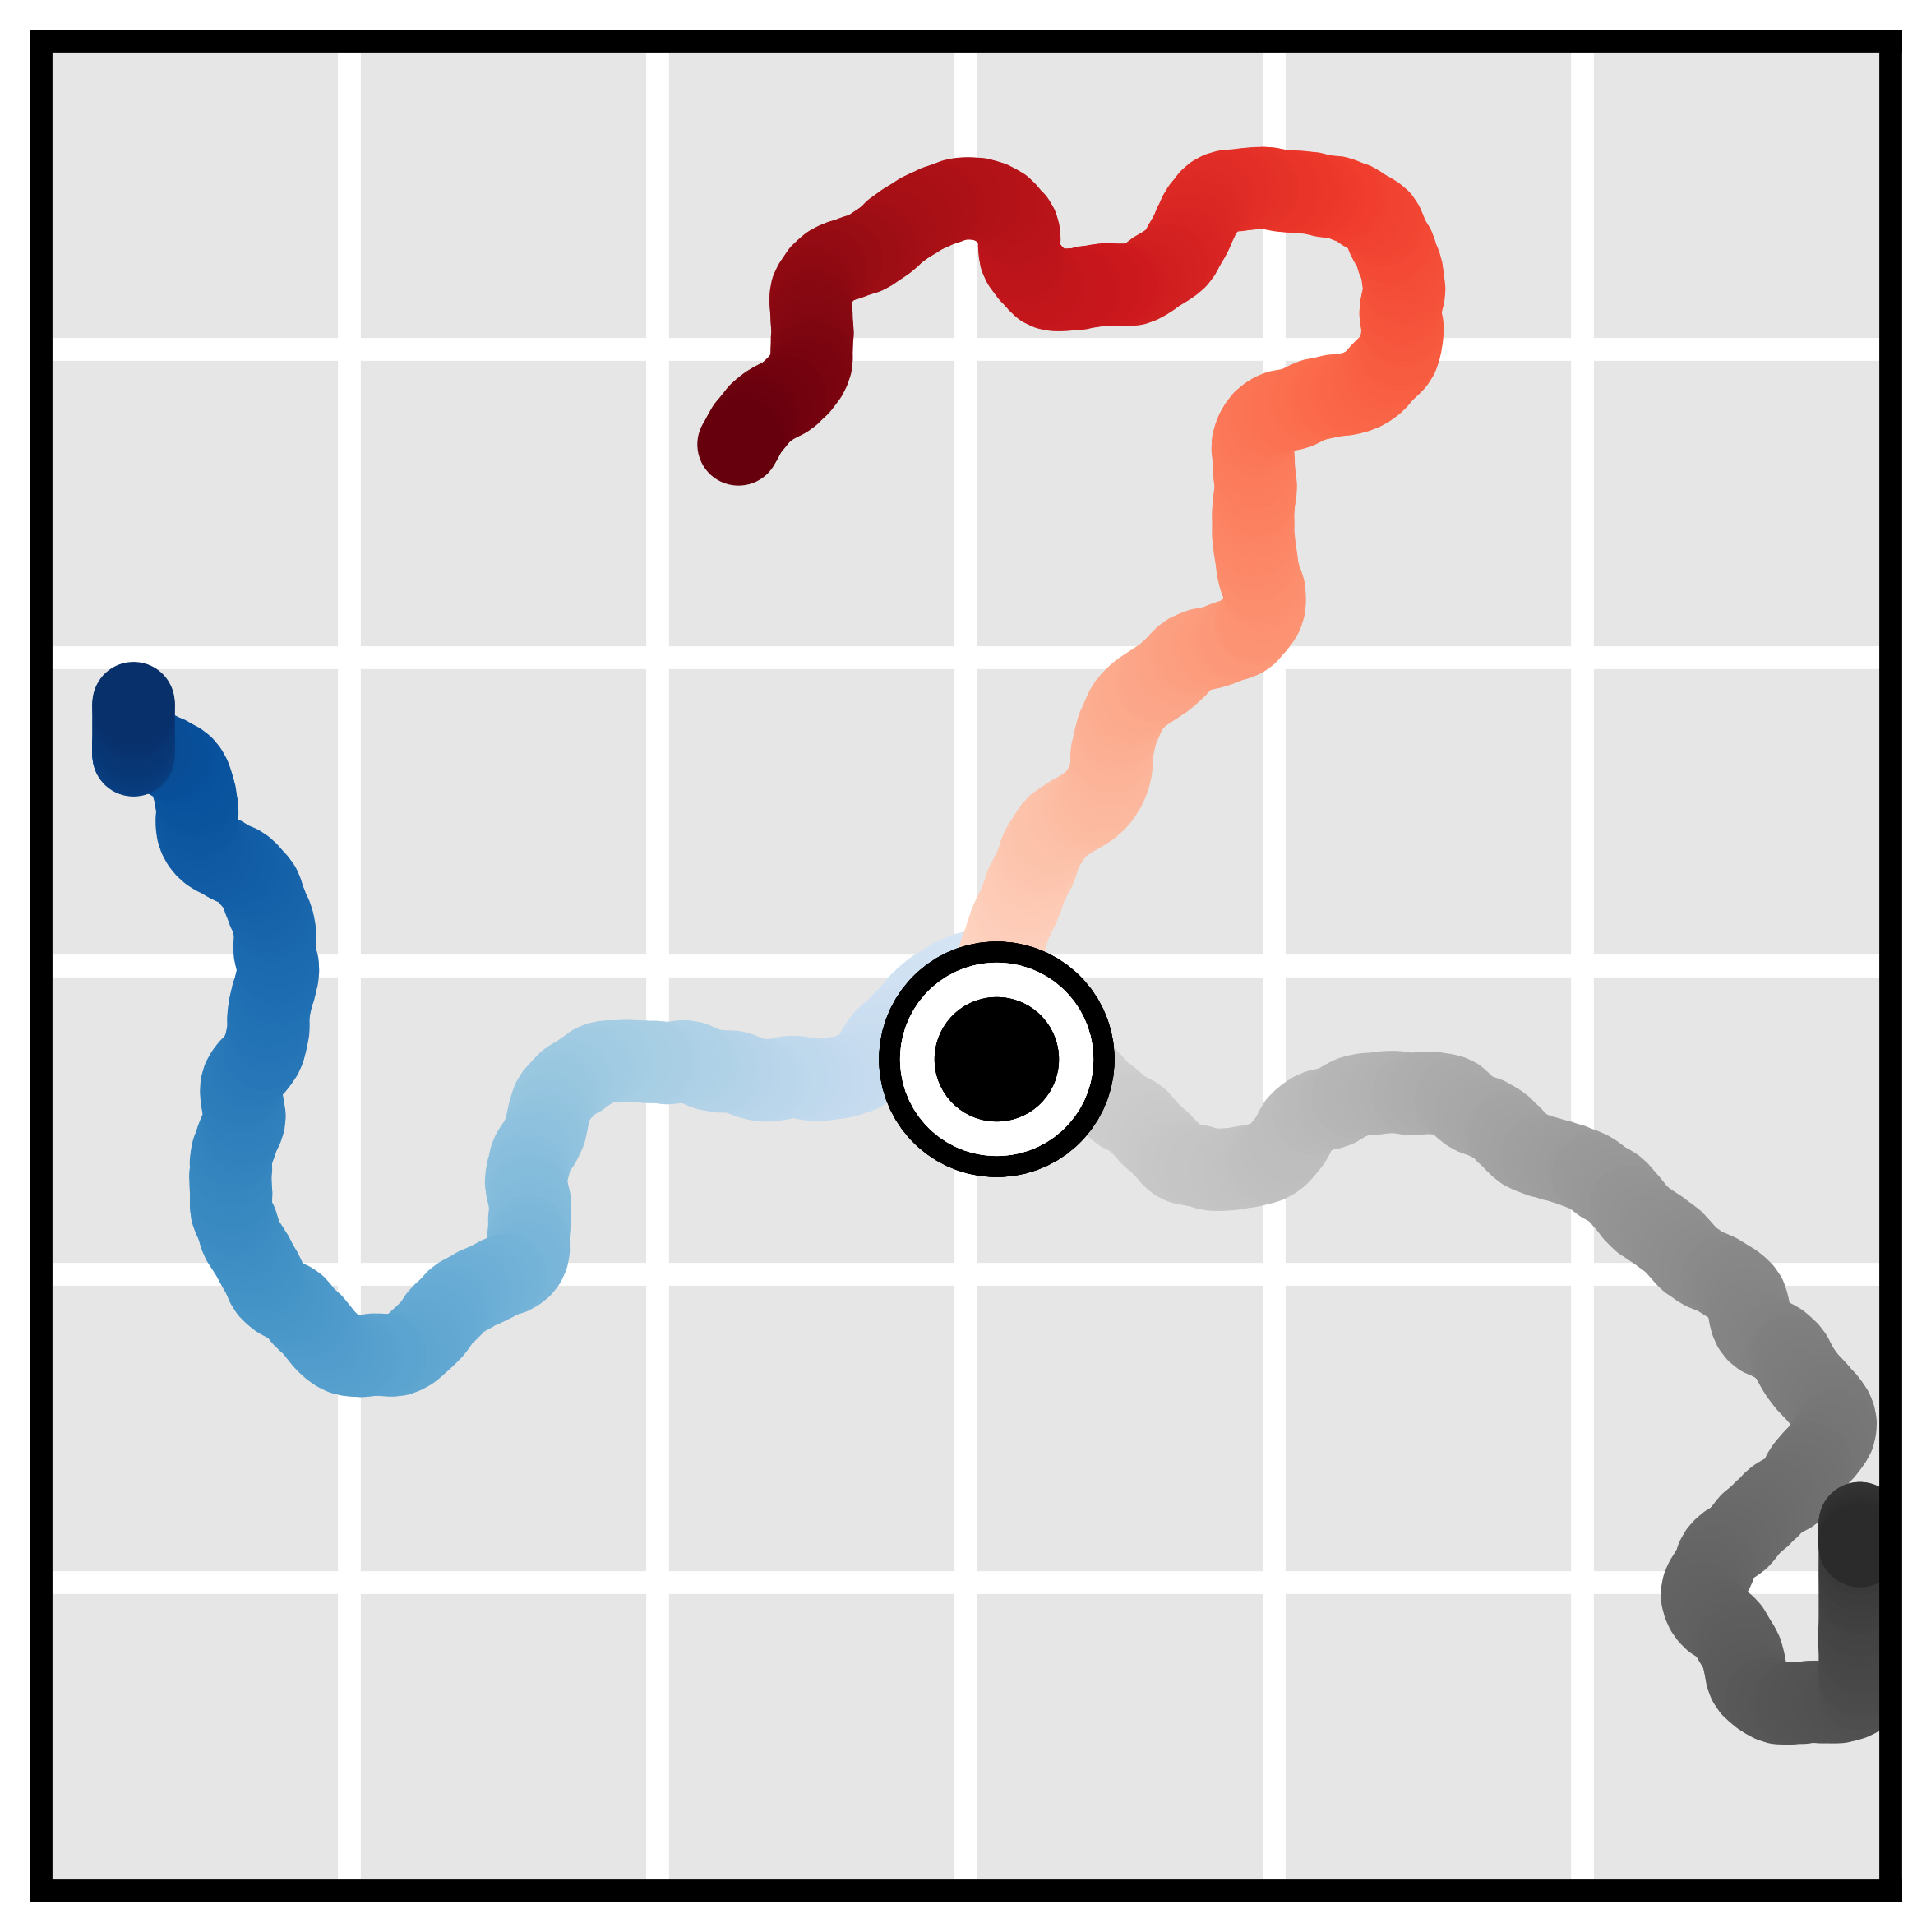
\includegraphics[width=2.5cm]{images/properties/variable_1_3.png} \\
    % ~~~~\raisebox{2cm}{$\btau{N}$} \\
\end{minipage}%
%%%%
\begin{minipage}[t]{0.35\textwidth}
    \raisebox{2cm}{\textbf{d}}~~~
    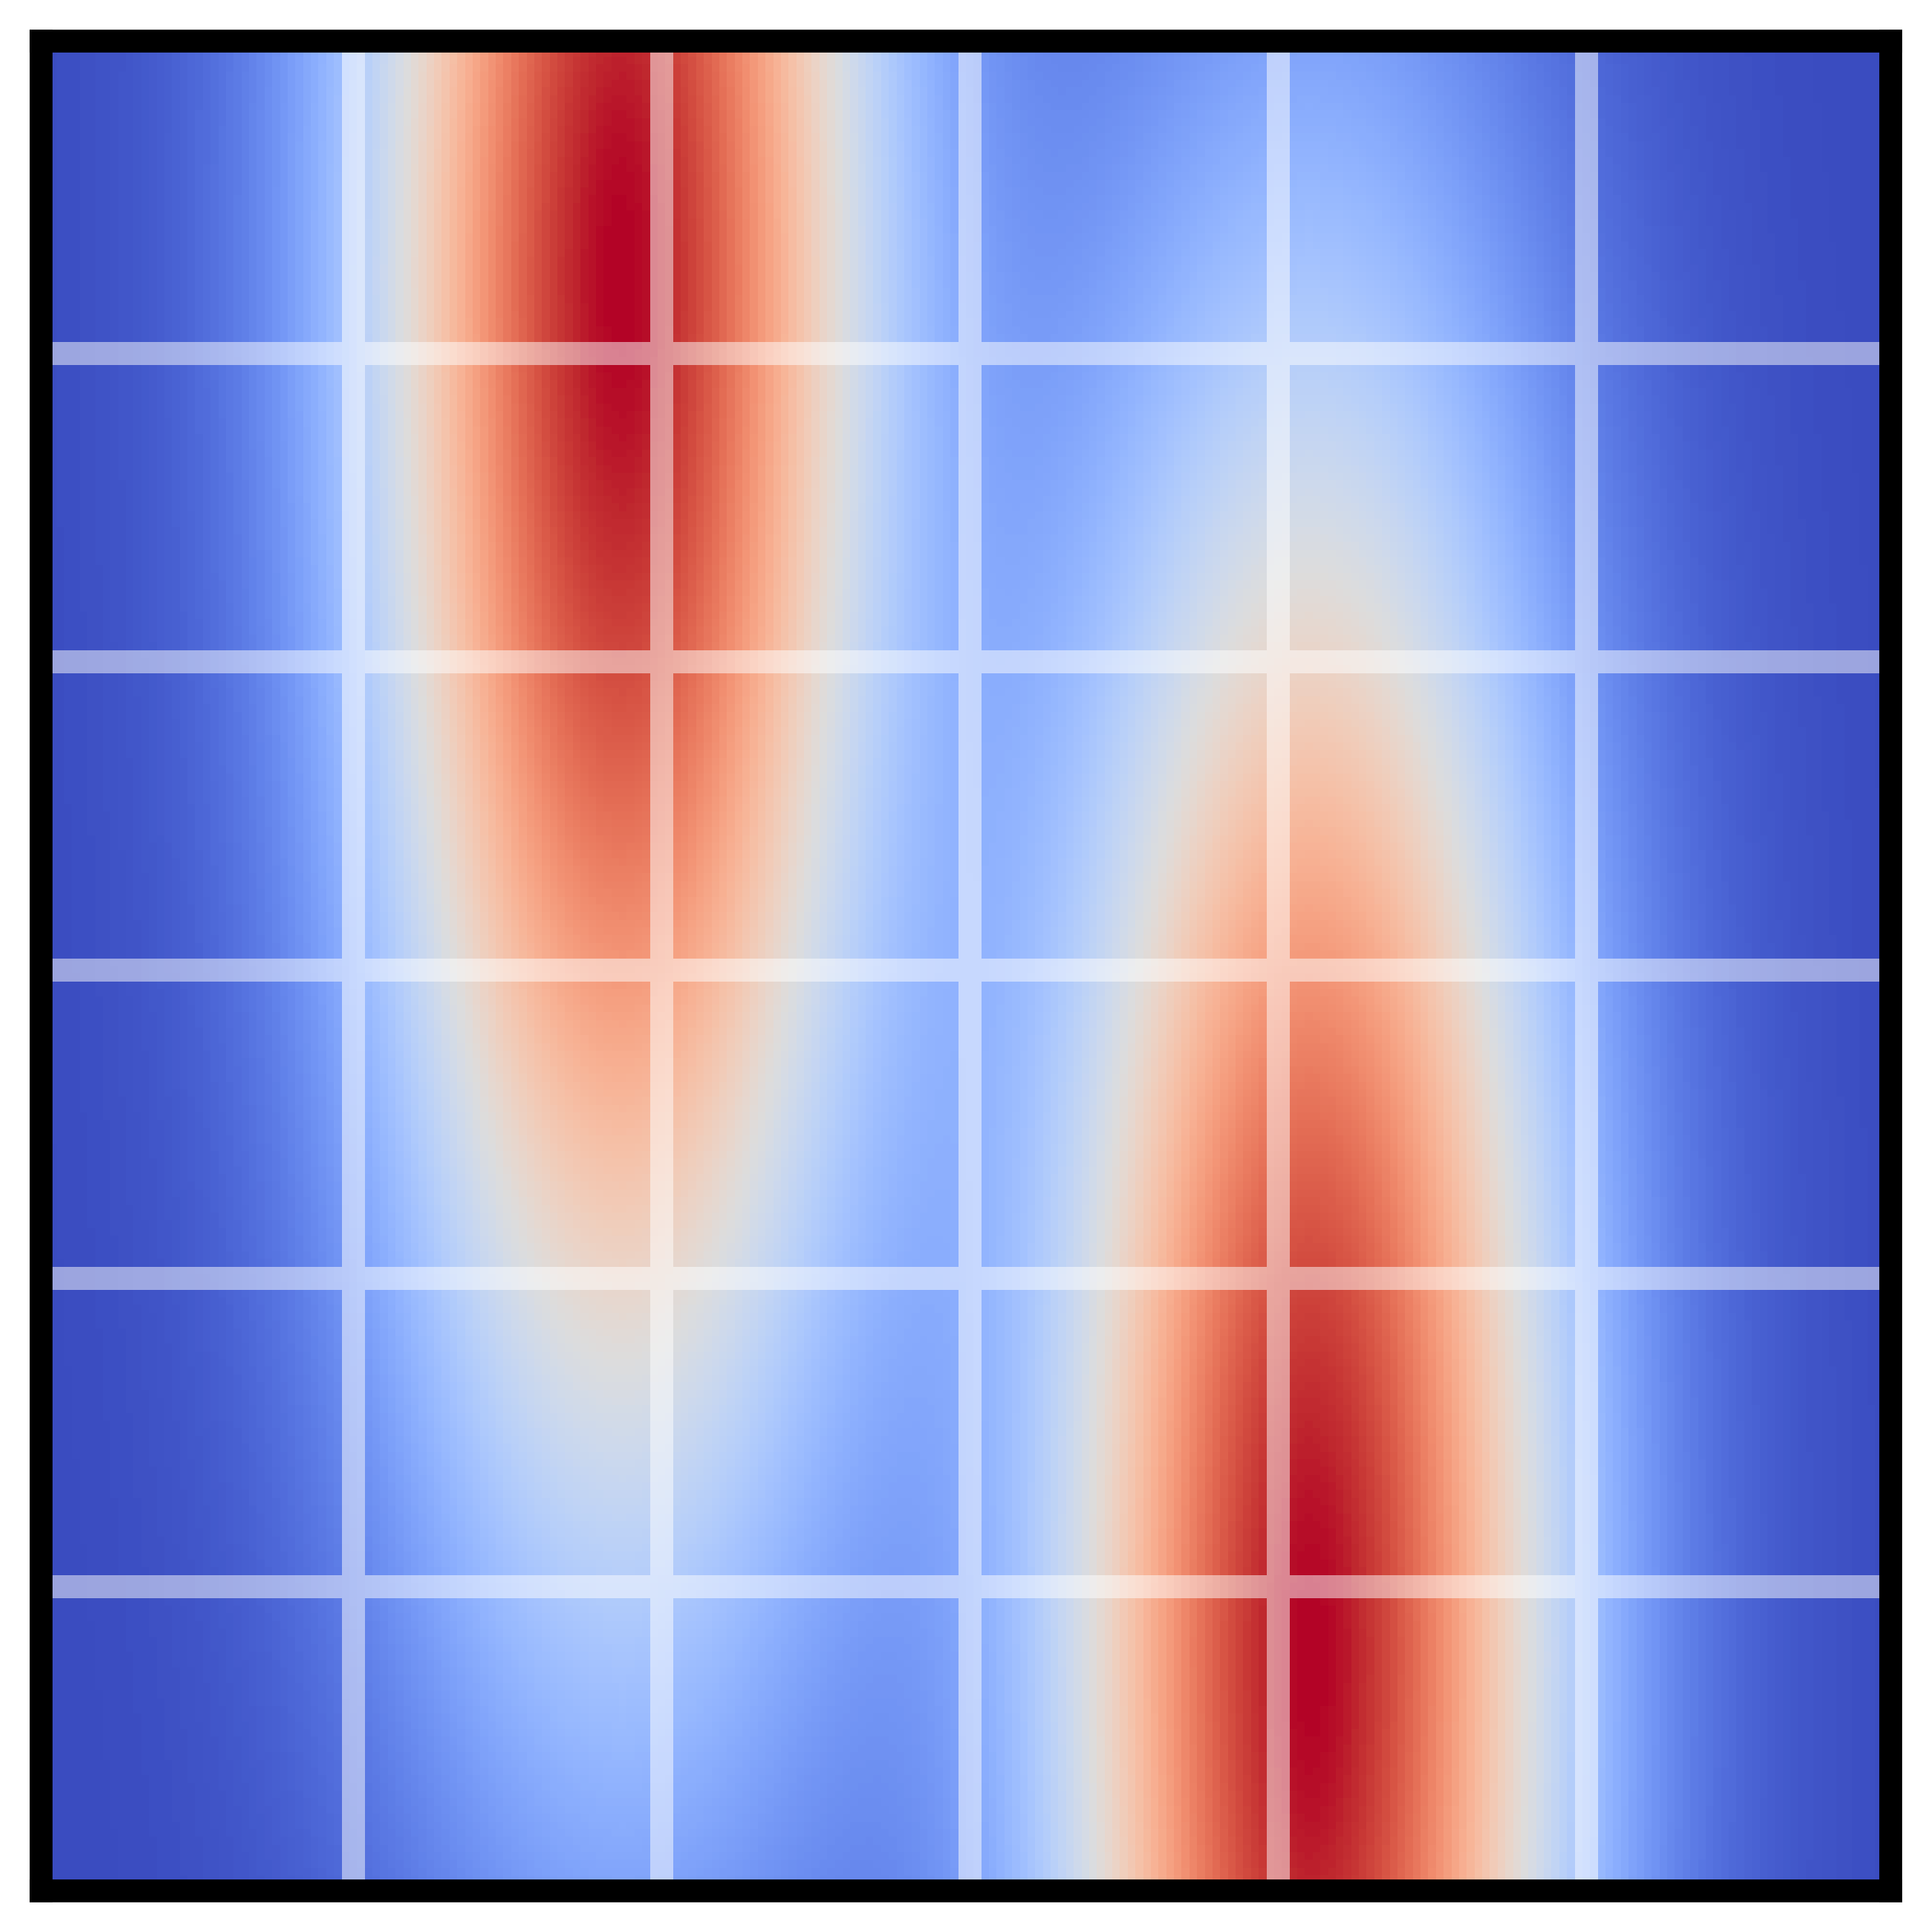
\includegraphics[width=2.5cm]{images/properties/reward.png}~
    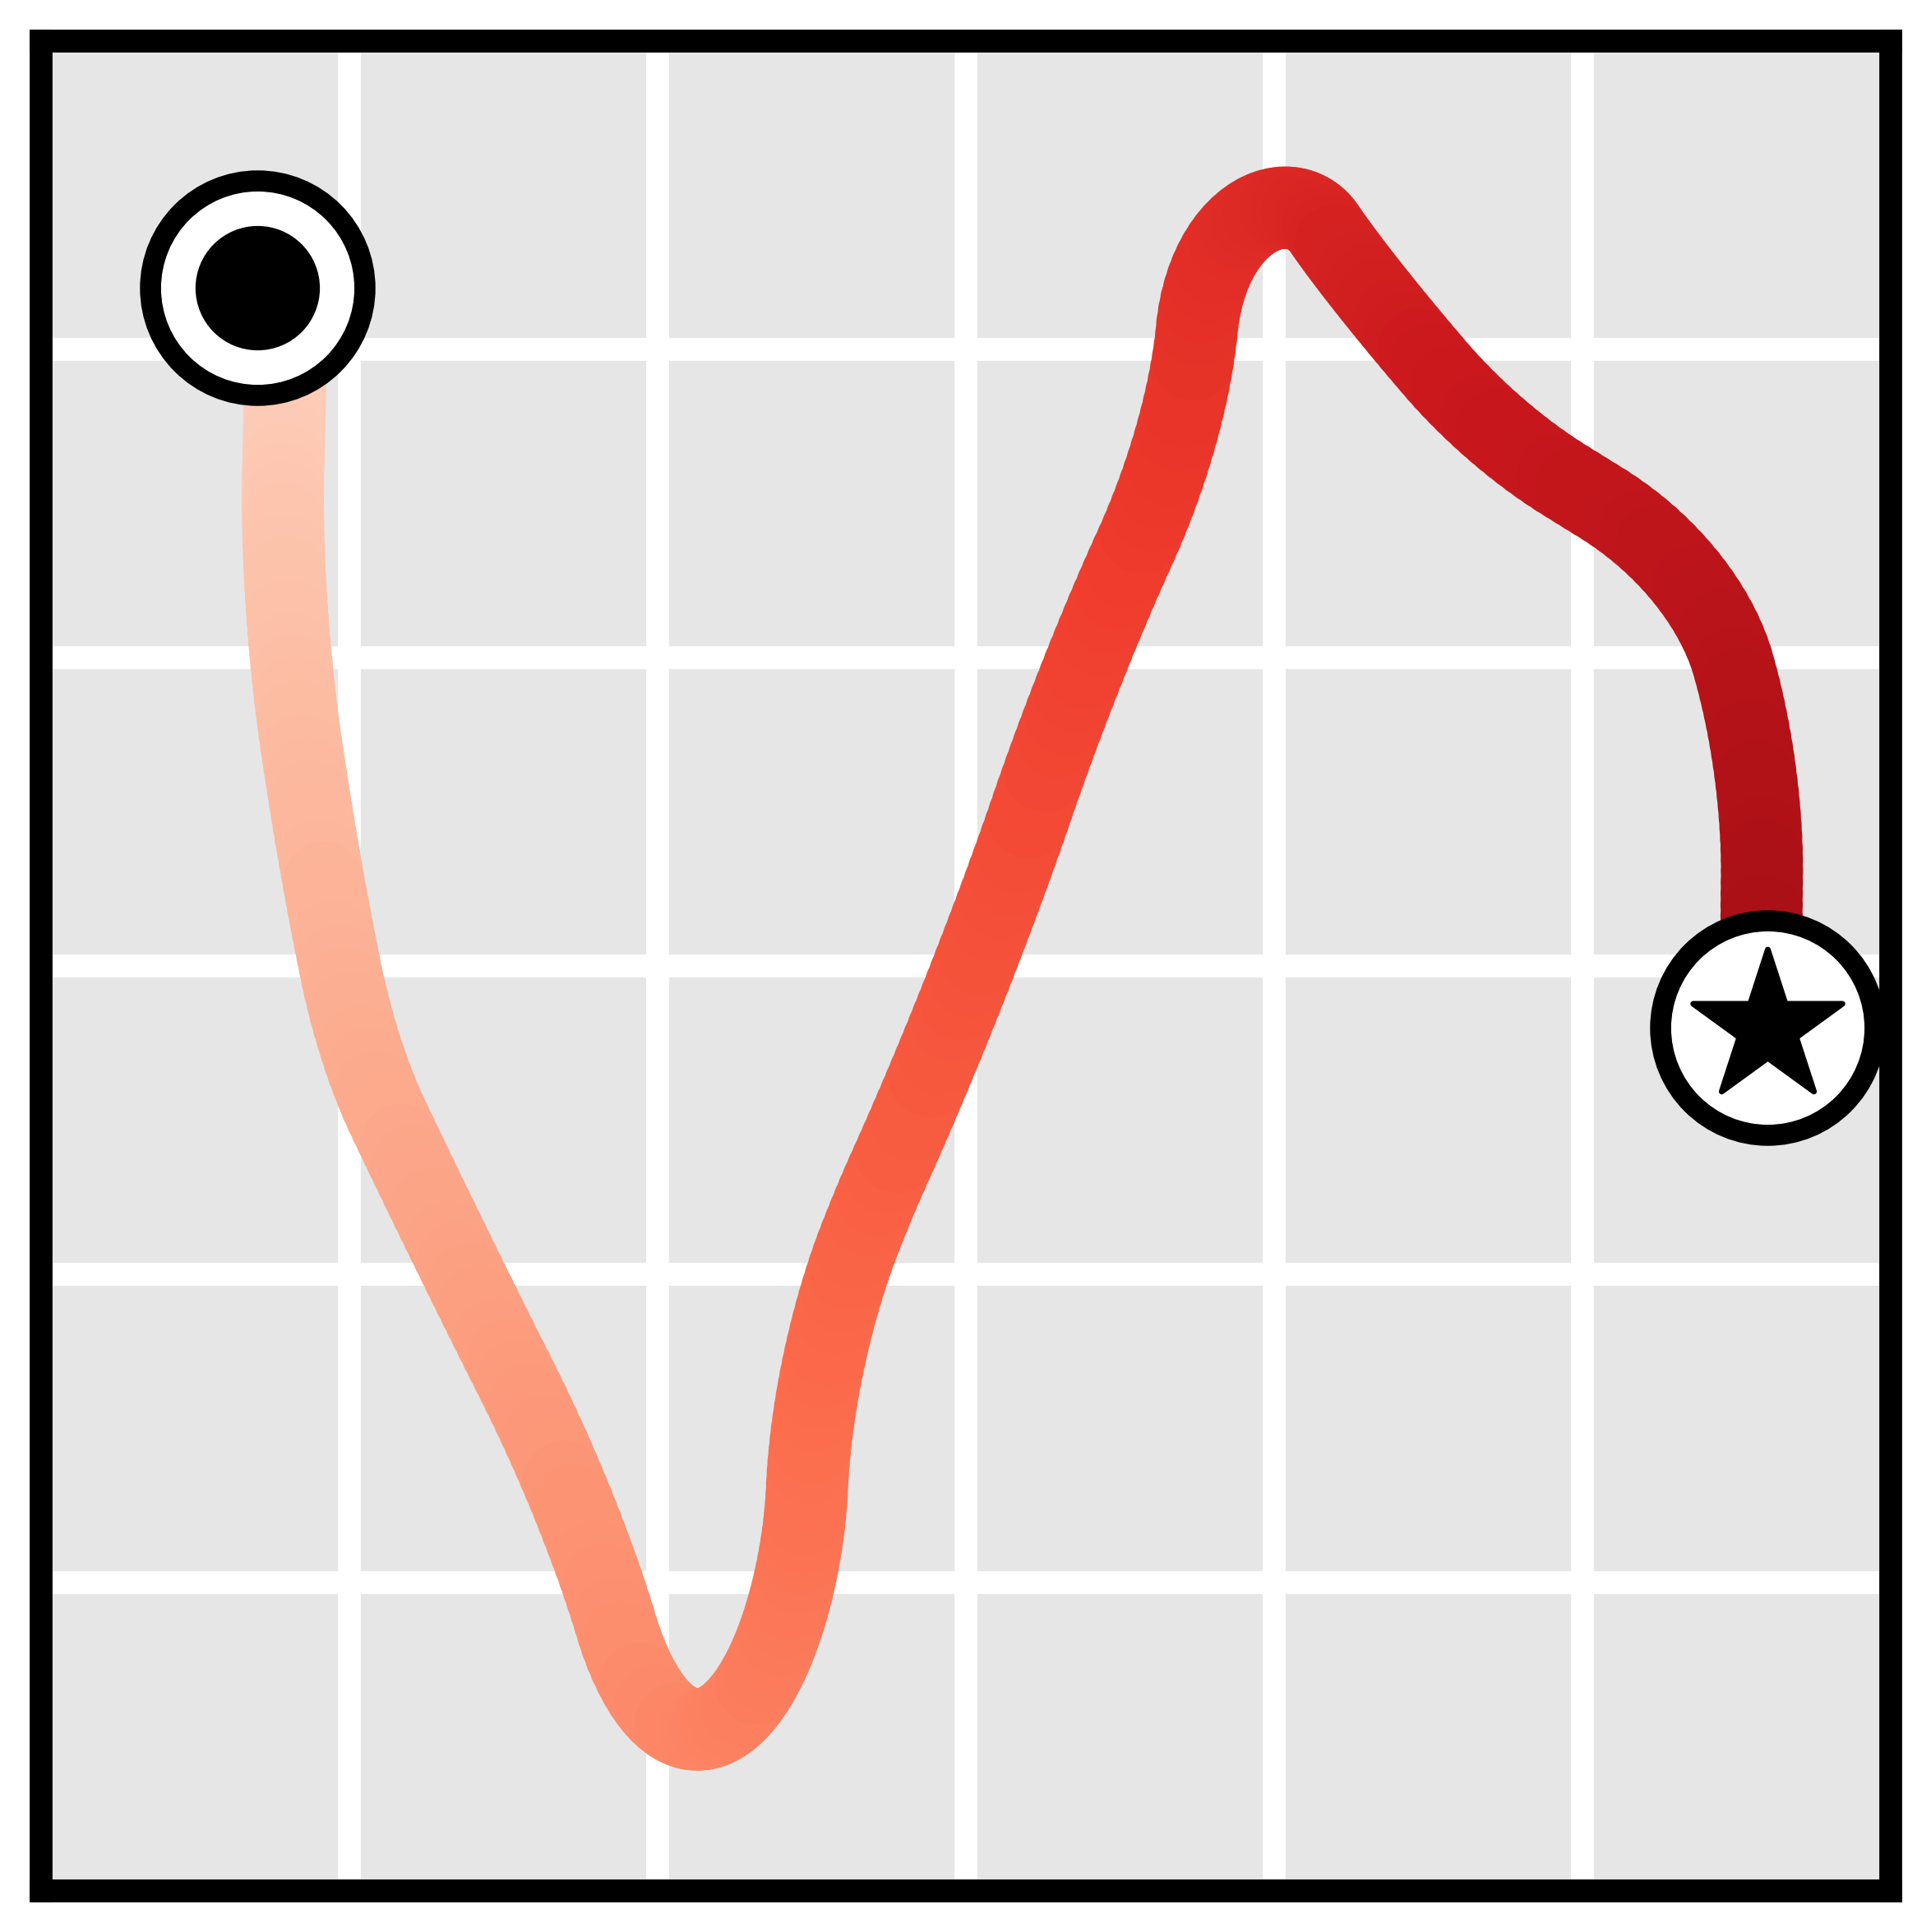
\includegraphics[width=2.5cm]{images/properties/reward_plan.png} \\
    \vspace{-.5cm}
    \begin{flushleft}
            \hspace{0.43cm} reward
            \hspace{0.0cm}
            \raisebox{.05cm}{$-$}
            \raisebox{.0cm}{
\includegraphics[height=1cm,angle=90]{images/properties/reward_colorbar.png}}
            \raisebox{.05cm}{$+$}
            \hspace{0.6cm} plan \\
    \end{flushleft}
\end{minipage}
\caption{
    % \small
    \textbf{(Properties of diffusion planners)}
    \textbf{(a) Learned long-horizon planning:}
    \method{}'s learned planning procedure does not suffer from the myopic failure modes common to shooting algorithms and is able to plan over long horizons with sparse reward.
    \textbf{(b) Temporal compositionality:} Even though the model is not Markovian, it generates trajectories via iterated refinements to local consistency.
    As a result, it exhibits the types of generalization usually associated with Markovian models, with the ability to stitch together snippets of trajectories from the training data to generate novel plan.
    \textbf{(c) Variable-length plans:}
    Despite being a trajectory-level model, \method's planning horizon is not determined by its architecture.
    The horizon can be updated after training by changing the dimensionality of the input noise.
    \textbf{(d) Task compositionality:} \method{} can be composed with new reward functions to plan for tasks unseen during training.
    In all subfigures,
    \protect{\raisebox{-.05cm}{
\includegraphics[height=.35cm]{images/maze2d/mark_start_crop.png}}}
    denotes a starting state and
    \protect{\raisebox{-.05cm}{
\includegraphics[height=.35cm]{images/maze2d/mark_goal_crop.png}}}
    denotes a goal state.
}
% \vspace{-.1cm}
\label{fig:properties}
% \vspace{-10pt}
\end{figure*}

% \section{Probabilistic Trajectory Optimization}
% \label{sec:method}


%%SL.1.5: I wonder if we can rephrase, as we are not just presenting "an implementation" but actually describing our method
% Next, we present our approach towards towards practically learn a trajectory optimization framework described in \sect{sect:traj_opt}. First, we discuss a framework reinterpreting trajectory optimization probablistically, and then discuss how to implement this framework using diffusion probabilistic models. 

% \subsection{Probabilistic Trajectory Optimization}
% \label{sec:prob_traj_opt}

% A difficulty of the trajectory optimization procedure in \sect{sect:traj_opt} is that it requires knowledge of the ground truth dynamics model $\vf$. While a significant amount of prior work has explored learning models of $\vf$, directly optimizing for a trajectory under a learned $\vf$ often leads to the construction of adversarial trajectories.

% To sidestep this issue of adversarial trajectories, we propose to directly learn a probabilistic model over trajectories $p_\text{traj}(\tau)$, and generate different trajectories $\tau$ from $p_\text{traj}(\tau)$ as opposed to rolling out the a learned model $\vf$.

% We then further construct a probabilistic analogue of  \eqn{eqn:cost_fns}, $q_\text{cost}(\bm{\tau}) = e^{-J(\bm{\tau})}$. This resultant distribution $q_\text{cost}(\bm{\tau})$ assigns high likelihood to distributions exhibiting low cost, and low likelihood to distributions exhibiting high cost. By composing both $p_\text{traj}(\bm{\tau})$ and $q_\text{cost}(\bm{\tau})$, we constructed a joint likelihood distribution $r_\text{opt}(\bm{\tau})$, and generate trajectories $\bm{\tau}$ by sampling from the this underlying probability distribution 
% \begin{equation}
%     \tau \sim r_\text{opt}(\bm{\tau}) = p_\text{traj}(\bm{\tau}) q_\text{cost}(\bm{\tau}).
%     \label{eqn:compose_traj_opt}
% \end{equation}

% This inference expression can be seen as an probabilistic analogue to \eqn{eqn:traj_opt}, as we simultaneously construct trajectories that are both high-likelihood under $p_\text{traj}(\bm{\tau})$ (are realistic trajectories) and which are high-likelihood under $q_\text{cost}(\bm{\tau})$ (exhibit low cost).

% While trajectory optimization enables the synthesis of flexible and adaptable behaviors, both $E_{dynamic}(\bm{\tau})$ and $E_{task}(\bm{\tau})$ are difficult to construct in unknown environments. In particular, the energy function $E_{dynamic}(\bm{\tau})$, requires knowledge of the underlying dynamics of the environment to construct while $E_{task}(\bm{\tau})$ requires ground truth knowledge of the underlying reward function/task.

% The key insight in this paper is that we may instead learn energy functions for both $E_{dynamics}$ and $E_{task}$ from trajectories from the environment.
% % $(\bs_1, \ba_1, \br_1, \bs_2, \ba_2, \br_2, \ldots, \bs_T, \ba_T, \br_T)$. 
% To learn a model of $E_{dynamics}$, we may utilize the underlying density of observed trajectories $p_{traj}(\bm{\tau})$ to define $E_{dynamics}$.  Given  $p_{traj}(\bm{\tau})$, we may  then treat $p_{traj}(\bm{\tau})$ as an EBM to obtain $p_{traj}(\bm{\tau}) = e^{-E_{dynamic}(\bm{\tau})}$. Our learned energy function $E_{dynamics}$ similarly penalizes trajectories with non-realistic dynamics, but does not require ground truth knowledge of dynamics of the environment.

% To learn $E_{task}(\bm{\tau})$, we may then utilize existing techniques from reinforcement learning to estimate the extent to which each trajectory completes a task using rewards at each individual time-step. \du{Michael add more clarification here?} In particular, we utilize Q learning to obtain a $E_{task}(\bm{\tau}) = -Q(\tau)$ to represent the underlying compatibility of a trajectory with a desired task.

% Given our learned energy functions $E_{dynamics}$ and $E_{task}$ and specified constraints $E_{const}$, we construct a probablistic analogue to the trajectory optimization procedure in \eqn{eqn:traj_opt}
% \begin{equation}
%   \bm{\tau}^* \sim e^{-(E_{dynamics}(\bm{\tau}) + E_{task}(\bm{\tau}) + E_{const}(\bm{\tau}))}, 
%   \label{eqn:prob_traj_opt}
% \end{equation}
%  to enable the sampling of a diverse set of different possible plans.
 
 
% Below, we describe a practical implementation of the probabilistic inference procedure utilizing diffusion probabilistic models. A related probabilistic formulation of trajectory optimization utilizing EBMs is described in \citep{du2019model}. In this paper, we provide a generic formulation of probabilistic trajectory optimization and validate our approach on more complex environments.


% \subsection{Diffusion Guided Trajectory Optimization}
% \label{sec:diffusion_traj_opt}

% We utilize a denoising diffusion probabilistic model to implement the probabilistic trajectory optimization in \eqn{eqn:compose_traj_opt}. We parameterize the probability distribution  $p_\text{traj}(\t)$ utilizing a set of marginal distributions
% \begin{equation}
%       p_\text{traj}(\t_{t-1} | \t_t) =  \mathcal{N}(\mu_\theta(\t_t, t), \sigma_t^2).
% \end{equation}

% We are then able to directly compose our distribution $p_\text{traj}(\t)$ with our specified costs $q_\text{cost}(\t)$
% to form the optimization distribution $r_\text{opt}(\t)$ utilizing a modified set of marginal distributions
% \begin{equation}
%   r_\text{opt}(\t_{t-1} | \t_t) =  \mathcal{N}(\mu_\theta(\t_t, t) - \lambda \nabla_{\t_t} J(\bm{\tau}), \sigma_t^2).
% \end{equation}

% \todo{Talk a bit about implementation details of the diffusion model? Could also maybe give pseudocode for execution?}